\documentclass[12pt]{report}

% \usepackage{setspace}
\usepackage[backend=biber, sorting=none]{biblatex}
\usepackage{graphicx}
\usepackage{dirtytalk}
\usepackage{geometry} 
\usepackage{tabulary}
\usepackage{listings}
\usepackage{setspace}
\usepackage{pdfpages}
\usepackage{subfiles}
    \geometry{
        a4paper,
        left=4cm,
        right=2.5cm,
        tmargin=2.5cm,
        bottom=2.5cm
    }

\doublespacing


\addbibresource{../bibliography/papers.bib}
\addbibresource{../bibliography/misc.bib}

\lstset{frame=single, basicstyle=\ttfamily}

\begin{document}

% \begin{titlepage}
\begingroup
    \centering
    {\Large\bfseries CHEFEED} \\
    {\large\bfseries DESIGNING SECURE MOBILE APPLICATIONS WITH OWASP SECURITY KNOWLEDGE FRAMEWORK}

    \vspace{1.5cm}
    
    {\large\bfseries THESIS \\ RESEARCH PROJECT}
    
    \vspace{1.5cm}
    
    {\large \textt{By}}

    \vspace{1.5cm}

    {\large\textit{Imanuel Febie 2201835800}}
    
    \begin{figure}[!h]
        \centering
        
\includegraphics[width=\textwidth]{img/binus-inter-logo.jpg}
    \end{figure}

    \vspace{1.5cm}

    {\normalize \bfseries BINUS International \\ BINUS UNIVERSITY \\ JAKARTA \\ 2022}

\endgroup
\end{titlepage}


% \subfile{preliminary_pages/approval}

% 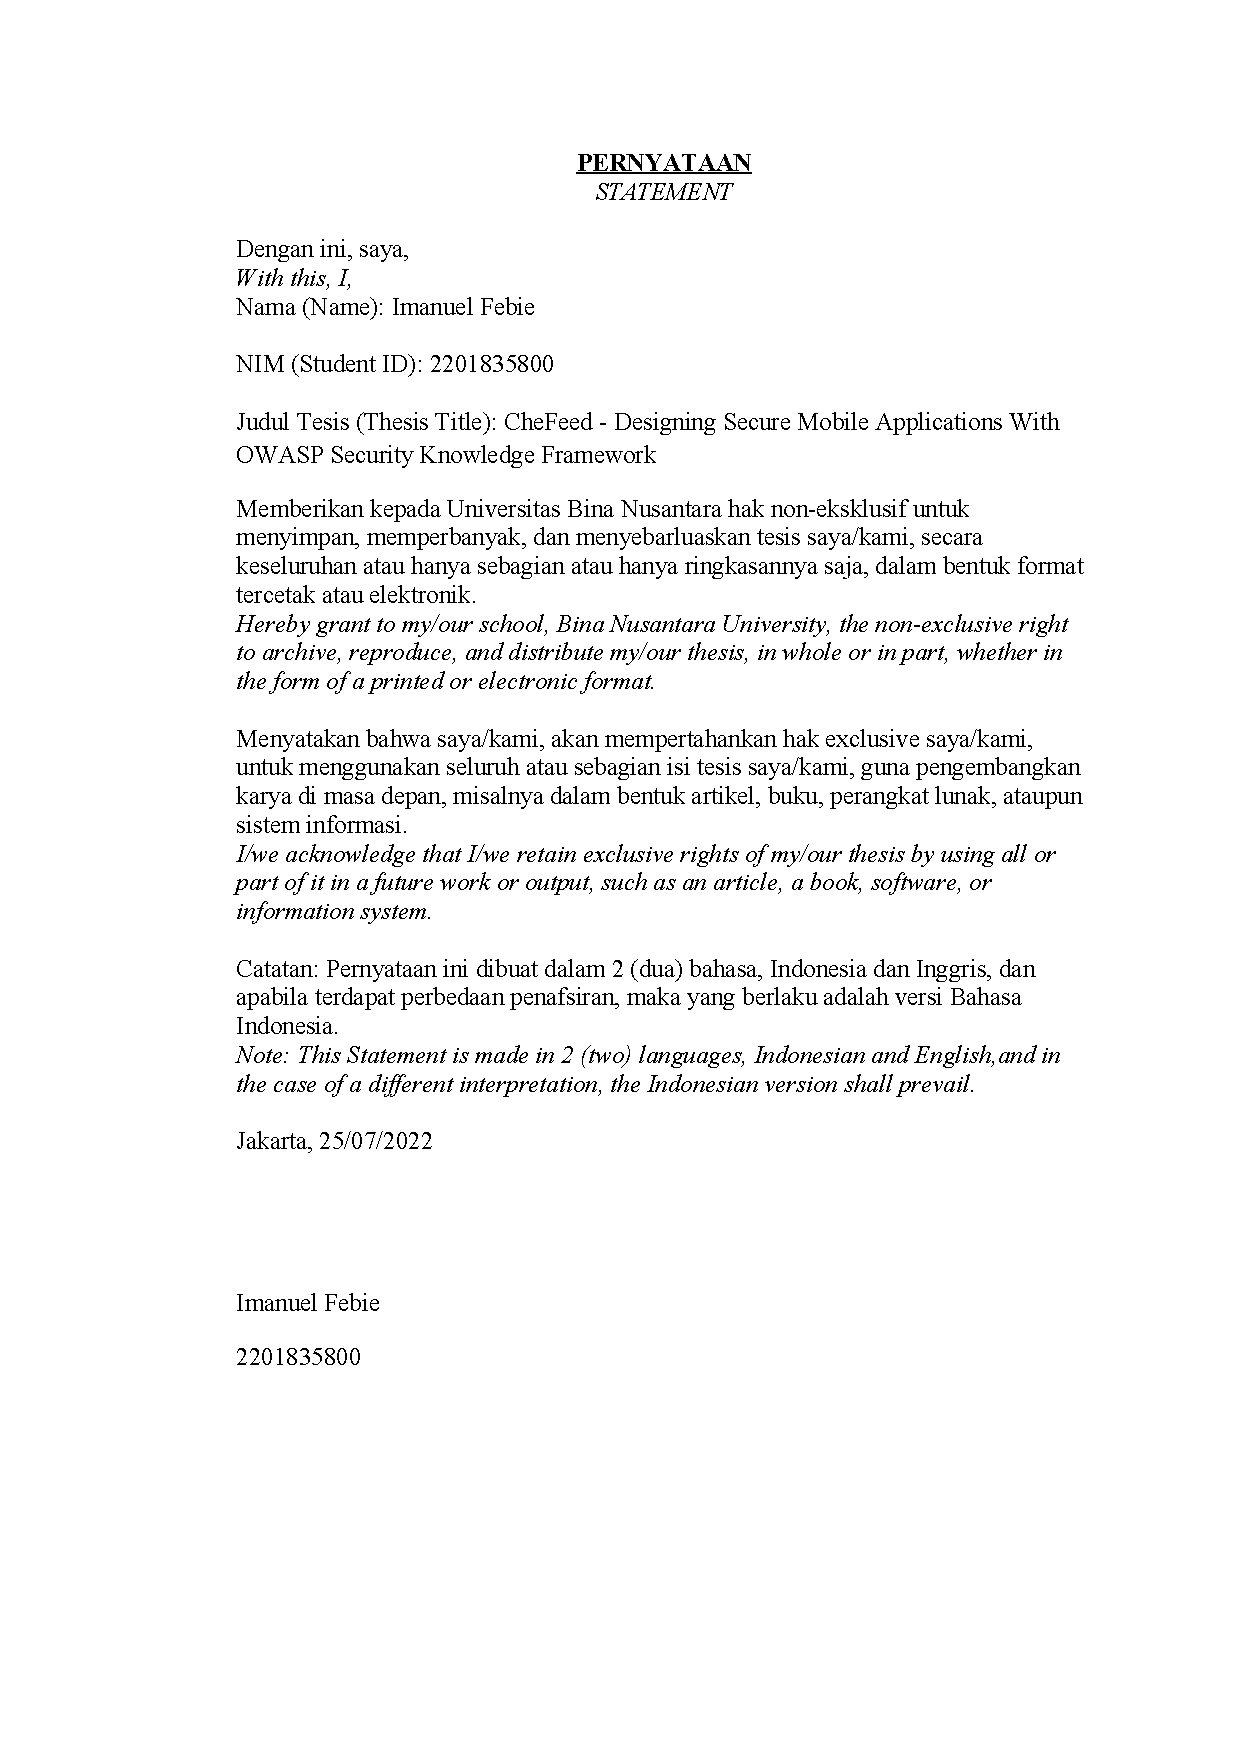
\includepdf{preliminary/statement.pdf}

% \subfile{chapters/0-abstract}

% \tableofcontents
% \listoffigures
% \listoftables

\chapter{Introduction}
\subfile{chapters/chapter-1}
% \subfile{chapters/chapter-1/1.1-background}
% \subfile{chapters/chapter-1/1.2-scope}
% \subfile{chapters/chapter-1/1.3-aims-and-benefits}
% \subfile{chapters/chapter-1/1.4-structures}

% \chapter{Theoretical Foundation}
% \subfile{chapters/chapter-2/2-chapter-introdution}
% \subfile{chapters/chapter-2/2.1-theoretical-foundation}
% \subfile{chapters/chapter-2/2.2-fundamentals-of-infosec}
% \subfile{chapters/chapter-2/2.3-software-development}
% \subfile{chapters/chapter-2/2.4-security-testing}

% \chapter{Analysis on Secure Software Development}\label{chap:3}
% \subfile{chapters/chapter-3/index}

% CHAPTER 4
% \chapter{Security Solution Design}
% \subfile{chapters/chapter-4/index}

% CHAPTER 5
% \chapter{Testing and Implementation}
% \subfile{chapters/chapter-5/index}

% CHAPTER 6
% \chapter{Evaluation}
% \subfile{chapters/chapter-6/index}


% CHAPTER 7
% \chapter{Conclusion and Recommendation}
% \subfile{chapters/chapter-7/index}

\printbibliography

\end{document}
